\documentclass{tufte-handout}

\usepackage{style}

\begin{document}

\tma{04} % TMA number

\section{Part A}

%Question 1
\begin{question}

\qpart

By \textup{Definition 1.9 Chapter 13 p63 and Theorem 1.22 Chapter 13 p 64};

\qsubpart

An example of a strictly monotonic decreasing sequence is;
\[ (x_n) = 1 + \frac{1}{n}, \text{ for } n \geq 1 \]

It is decreasing because;
\begin{align*}
x_{n+1} - x_n &= \left( 1 + \frac{1}{n+1} \right) - \left( 1 + \frac{1}{n} \right) \\[8pt]
&= \frac{1}{n+1} - \frac{1}{n}\\[8pt]
&= \frac{n - (n+1)}{n(n+1)} \\[8pt]
&= \frac{-1}{n(n+1)} < 0\\[8pt]
\snote{for all \( n \geq 1 \)}
\end{align*}

and,

\[ \lim\limits_{n \to \infty} x_n = \lim\limits_{n \to \infty} \left( 1 + \frac{1}{n} \right) = 1 + 0 = 1 \]

Since \( (x_n) \) is strictly monotonic decreasing and bounded below by 1, it converges, \textup{Theorem 1.22 HB Chapter 13 p64}, 
and from the above we see that,

\[ \lim\limits_{n \to \infty} x_n = 1 \]

\vspace{2cm}

\qsubpart

An example of a strictly monotonic increasing sequence is;
\[ (y_n) = -1 - \frac{1}{n}, \text{ for } n \geq 1 \]

It is increasing because;
\begin{align*}
y_{n+1} - y_n &= \left( -1 - \frac{1}{n+1} \right) - \left( -1 - \frac{1}{n} \right) \\[8pt]
&= - \frac{1}{n+1} + \frac{1}{n} \\[8pt]
&= \frac{-n + (n+1)}{n(n+1)} \\[8pt]
&= \frac{1}{n(n+1)} > 0\\[8pt]
\snote{for all \( n \geq 1 \)}
\end{align*}    

and,

\[ \lim\limits_{n \to \infty} y_n = \lim\limits_{n \to \infty} \left( -1 - \frac{1}{n} \right) = -1 - 0 = -1 \]

Since \( (y_n) \) is strictly monotonic increasing and bounded above by -1, it converges, \textup{Theorem 1.22 HB Chapter 13 p64},
and from the above we see that,

\[ \lim\limits_{n \to \infty} y_n = -1 \]

\vspace{2cm}

\qpart

\begin{equation*}
    (z_n) =
\begin{cases}
 x_n, & \text{if } n \text{ is odd}\\
 y_n, & \text{if } n \text{ is even}
\end{cases}
\end{equation*}

Using \textup{Definition 1.24 HB Chapter 13 p65}, where \( (x_n) \) is the strictly monotonic decreasing sequence defined 
in part (a)(i) and \( (y_n) \) is the strictly monotonic increasing sequence defined in part (a)(ii).
We can see that the subsequence of odd terms \( (z_{2n-1}) \) is equivalent to \( (x_n) \) and the subsequence of even 
terms \( (z_{2n}) \) is equivalent to \( (y_n) \).
Thus we have that;
\[\lim\limits_{n \to \infty} z_{2n-1} = \lim\limits_{n \to \infty} x_n = 1 \]
and
\[\lim\limits_{n \to \infty} z_{2n} = \lim\limits_{n \to \infty} y_n = -1 \]
Since the two subsequences converge to different limits, and by \textup{Proposition 1.25 HB Chapter 13 p65}, the sequence \( (z_n) \) does not converge.

\end{question}

%Question 2

\begin{question}

\[ L = \bm{L_{a,\theta}} = \{ (x,a+x\tan\theta):x \in \R \} \]

Where \( a \) is the y- intercept of the line and \( \theta \) is the angle of inclination of the line to the positive x-axis.

\[ \mathbf{X} =  \bm{L_{a,\theta}} : \mathbf{a} \in \R \text{ and } \theta \in (-\pi/2, \pi/2)  \]

and the distance function;

\[ \Delta(\bm{L_{a,\theta}}, \bm{L_{b,\phi}}) = \mid a-b \mid + \mid \tan{\theta} - \tan{\phi} \mid \]
for \( \bm{L_{a,\theta}}, \bm{L_{b,\phi}} \in \mathbf{X} \)

\qpart

The distance between \( \bm{L_{0,\pi/4}} \text{ and } \bm{L_{1,-\pi/4}} \);

\begin{align*}
\bm{\Delta(L_{0,\pi/4}, L_{1,-\pi/4})} &= \mid 0-1 \mid + \mid \tan{\pi/4} - \tan{-\pi/4} \mid \\[8pt]
&= 1 + \mid 1 - (-1) \mid \\[8pt]
&= 1 + \mid 2 \mid \\[8pt]
&= 1 + 2 = 3
\end{align*}

\vspace{2cm}

\qpart

By \textup{Definition 2.1, HB Chapter 14 p72},

\qsubpart

To show \( \Delta \) satisfies (M1) non-negativity, we need to show that for all \( \bm{(L_{a,\theta,L_{b,\phi} \in X})} \), 
\[ \bm{\Delta(L_{a,\theta,L_{b,\phi}})} \geq 0 \]

\begin{align*}
\Delta(\bm{L_{a,\theta}}, \bm{L_{b,\phi}}) &= \mid a-b \mid + \mid \tan{\theta} - \tan{\phi} \mid \\[8pt]
\stext{As \( \mathbf{a,b} \in \R \) and \( \theta \in (-\pi/2, \pi/2) \), both \( \mid a-b \mid \geq 0 \) and \( \mid \tan{\theta} - \tan{\phi} \mid \geq 0 \)} \\[8pt]
\stext{Hence}
\bm{\Delta(L_{a,\theta}, L_{b,\phi})} &\geq 0
\end{align*}

So, \( \Delta(\bm{L_{a,\theta}}, \bm{L_{b,\phi}}) \geq 0 \) and thus \( \bm{\Delta} \) is non-negative.

If 

\begin{align*}
\bm{\Delta(L_{a,\theta},L_{b,\phi})} &= \mid a - a \mid + \mid \tan{\theta} - \tan{\theta}\\[8pt]
&= 0 + 0 = 0
\end{align*}

and

\begin{align*}
\bm{\Delta(L_{a,\theta},L_{b,\phi})} &= 0 \\[8pt]
\stext{then} \mid a - b \mid + \mid \tan{\theta} - \tan{\phi} \mid &= 0 \\[8pt]
\stext{Since both terms are non-negative, they must both be zero, so} 
\mid a - b \mid &= 0 \text{ and } \mid \tan{\theta} - \tan{\phi} \mid = 0 \\[8pt]
\stext{which implies} 
a &= b \text{ and } \tan{\theta} = \tan{\phi} \\[8pt]
\stext{and since \( \theta, \phi \in (-\pi/2, \pi/2) \),} \theta &= \phi
\end{align*}

Thus, \( \bm{\Delta(L_{a,\theta}, L_{b,\phi})} = 0 \) if and only if \( a = b \) and \( \theta = \phi \), so (M1) is satisfied.


\vspace{2cm}

\qsubpart

To show \( \Delta \) satisfies (M2) symmetry, we need to show that for any
\( \bm{\Delta(a,b)} = \bm{\Delta(b,a)} \)

\begin{align*}
\bm{\Delta(L_{a,\theta}, L_{b,\phi})} &= \mid a-b \mid + \mid \tan{\theta} - \tan{\phi} \mid \\[8pt]
\stext{By the properties of absolute values, HB p8, \( \mid a-b \mid = \mid b-a \mid \) and \( \mid \tan{\theta} - \tan{\phi} \mid = \mid \tan{\phi} - \tan{\theta} \mid \)} \\[8pt]
&= \mid b-a \mid + \mid \tan{\phi} - \tan{\theta} \mid \\[8pt]
&= \bm{\Delta(L_{b,\phi}, L_{a,\theta})}
\end{align*}

Thus, \( \bm{\Delta(L_{a,\theta}, L_{b,\phi})} = \bm{\Delta(L_{b,\phi}, L_{a,\theta})} \) and (M2) is satisfied.

\vspace{2cm}

\qsubpart

To show \( \Delta \) satisfies (M3) triangle inequality, we need to show that for any
\( \bm{\Delta(a,c)} \leq \bm{\Delta(a,b) + \Delta(b,c)} \)

\begin{align*}
\bm{\Delta(L_{a,\theta}, L_{c,\psi})} &= \mid a-c \mid + \mid \tan{\theta} - \tan{\psi} \mid \\[8pt]
\stext{By the triangle inequality for real numbers, HB p9,}
&\leq \left( \mid a-b \mid + \mid b-c \mid \right) + \left( \mid \tan{\theta} - \tan{\phi} \mid + \mid \tan{\phi} - \tan{\psi} \mid \right) \\[8pt]
\stext{Since}
\mid a - c \mid &\leq \mid a - b \mid + \mid b - c \mid\\[8pt]
\stext{And}
\mid \tan{\theta} - \tan{\psi} \mid \leq &\mid \tan{\theta} - \tan{\phi} \mid + \mid \tan{\phi} - \tan{\psi} \mid\\[8pt]
&= \mid a-b \mid + \mid \tan{\theta} - \tan{\phi} \mid + \mid b-c \mid + \mid \tan{\phi} - \tan{\psi} \mid \\[8pt]
\end{align*}

Thus, using the triangle inequality twice, \( \bm{\Delta(L_{a,\theta}, L_{c, \psi})} \leq \bm{\Delta(L_{a,\theta}, L_{b,\phi})} + \bm{\Delta(L_{b,\phi}, L_{c, \psi})} \) and (M3) is satisfied.

\vspace{5cm}

\qpart

\[ \mathbf{B_{\Delta}}(\mathbf{L_{0,0}},1) \]

By \textup{Definition 2.6, HB Chapter 14 p72} for open balls in a metric space, we have that, 

\begin{align*}
\mathbf{B_{\Delta}}(\mathbf{L_{0,0}},1) &= \{ \bm{L_{b,\theta}} \in \mathbf{X} : \Delta(\mathbf{L_{0,0}}, \bm{L_{b,\theta}}) < 1 \} \\[8pt]
&= \{ \bm{L_{b,\theta}} \in \mathbf{X} : \mid 0-b \mid + \mid \tan{0} - \tan{\theta} \mid < 1 \} \\[8pt]
&= \{ \bm{L_{b,\theta}} \in \mathbf{X} : \mid b \mid + \mid 0 - \tan{\theta} \mid < 1 \} \\[8pt]
&= \{ \bm{L_{b,\theta}} \in \mathbf{X} : \mid b \mid + \mid \tan{\theta} \mid < 1 \}
\end{align*}

\vspace{2cm}

\qpart

The sequence of lines;
\[ (\mathbf{L_{n}})_{n=1}^{\infty} \text{ given by } \mathbf{L_{n}} = \mathbf{L}_{-1/n,\pi/2-1/n} \]
is not \( \Delta-convergent \) because, by \textup{Definition 3.2 HB Chapter 14 p73};

\begin{align*}
\stext{Using \(\bm{L_{b,\phi}} \in \mathbf{X} \) Then}
\Delta(\mathbf{L_n}, \bm{L_{b,\phi}}) &= \left|-\frac{1}{n} - b\right|+ \left|\tan\left(\frac{\pi}{2}-\frac{1}{n}\right) - \tan\phi\right| \\[8pt]
\stext{As \(n \to \infty\), we have \(-1/n \to 0\), so}
\left|-\frac{1}{n} - b\right| \to |b|\\[8pt]
\stext{Also, as \(n \to \infty\), we have}
\tan\left(\frac{\pi}{2}-\frac{1}{n}\right) \to +\infty \\[8pt]
\stext{and since \(\tan\phi\) is finite for all \(\phi \in (-\pi/2,\pi/2)\),}
\left|\tan\left(\frac{\pi}{2}-\frac{1}{n}\right) - \tan\phi\right| \to \infty.
\end{align*}

Hence \(\bm{\Delta(L_n, L_{b,\phi})} \to \infty\), and so
\((\mathbf{L_n})\) is not \(\bm{\Delta}\)-convergent.

\end{question}


%Question 3
\begin{question}

\begin{equation*}
f_{n}(x) = 
\begin{cases}
\sin(\pi x), \text{ if } 2n \leq x < (2n+1),\\
0, \text{ otherwise. }
\end{cases}
\end{equation*}

\qpart

\fnSketch{1} % bump on [2π,3π)

\fnSketch{2} % bump on [4π,5π)

\fnSketch{3} % bump on [6π,7π)



\qpart

To test for pointwise limits we can take \( x = 2.5 \) as a constant value.

\begin{align*}
\stext{When \( n=1 \) the interval is \( [2,3) \)}
f_1(2.5) &= \sin(2.5\pi) = 1\\[8pt]
\stext{When \( n=2 \) the interval is \( [4,5) \)}
f_2(2.5) &= 0\\[8pt]
\stext{When \( n=3 \) the interval is \( [6,7) \)}
f_3(2.5) &= 0\\[8pt]
&\vdots \\[8pt]
\stext{When \( n=k \) the interval is \( [2k,2k+1) \)}
f_k(2.5) &= 0\\[8pt]
\end{align*}

By the Archimedean property, for any value of \( x \) there exists a natural number \( N \in \N \) such that \( 2N > x \).

Then for any \( n > N, \quad 2n > x \) and so \( f_{n} = 0 \). 

It follows that \( f_{x}(x) \to 0 \).

And so we conclude that the sequence \( (f_n) \) has a pointwise limit function \( f \), given by;

\[ f(x) = 0 \text{ for all } x \in \R \]

\vspace{3cm}

\qpart


Using \textup{Definition 4.4 Chapter 15 p 78} we can test for uniform convergence.


\begin{align*}
\forall n \in \R, \mid f_{n(x) - f(x) \mid} &= \mid f_{n}(x) - 0 \mid \\[8pt]
&= \mid f_{n}(x) \mid \\[8pt]
&= \begin{cases}
\mid \sin(\pi x) \mid, \text{ if } 2n \leq x < (2n+1),\\
0, \text{ otherwise. }
\end{cases}
\stext{Hence}
\sup_{x \in \R} \mid f_{n}(x) - f(x) \mid &= \sup_{x \in \R} \mid f_{n}(x) \mid \\[8pt]
&= \sup_{x \in [2n, 2n+1)} \mid \sin(\pi x) \mid \\[8pt]
&= 1
\end{align*}

It follows that \( f_{n} \) is not a null sequence of functions, and so \( f_{n} \) does not converge uniformly to \( f \text{ as } n \to \infty \)



\end{question}

%Question 4

\begin{question}
    
 \[ F : C[0,1] \to C[0,1] \]

    \[ F(f)(t) = \int_{t}^{1}(1 - x^4)f(x) \dd{x} \text{ for each } f \in C[0,1] \text{ and } t \in [0,1] \]

Let \( f \in C[0,1] \) and \( s,t \in [0,1] \) with \( s \leq t \).

Let \( f,g \in C[0,1] \) and \( t \in [0,1] \).

\begin{align*}
|F(f)(t) - F(g)(t)| &= \left| \int_{t}^{1}(1 - x^4)f(x) \dd{x} - \int_{t}^{1}(1 - x^4)g(x) \dd{x} \right| \\[8pt]
&= \left| \int_{t}^{1}(1 - x^4)(f(x) - g(x)) \dd{x} \right| \\[8pt]
&\leq \int_{t}^{1} |(1 - x^4)(f(x) - g(x))| \dd{x} \\[8pt]
&\leq \int_{t}^{1} (1 - x^4) |f(x) - g(x)| \dd{x} \\[8pt] 
\stext{Since \( 0 \leq (1-x^4) \leq 1  \forall  x \in [0,1] \)} \\[8pt]
&\leq \int_{t}^{1} |f(x) - g(x)| \dd{x} \\[8pt]
\stext{By Definition 5.1 HB Chapter 15 p79}
&\leq  d_{max}(f,g) \forall x \in [0,1] \\[8pt]
\stext{Hence}
&\leq \int_{t}^{1} d_{max}(f,g) \dd{x} = d_{max}(f,g)(1 - t) \\[8pt]
&\leq d_{max}(f,g) \\[8pt]
\stext{Taking the supremum over \( t \in [0,1] \) on the left hand side}
&= \sup_{t \in [0,1]} \mid F(f)(t) - F(g)(t) \mid \leq d_{max} \\[8pt]
\end{align*}

Hence \( F \) is a \( d_{max},d_{max} \)-Lipschitz function on \( C[0,1] \). 
Thus \( F \) is continuous by \textup{Theorem 3.2 Chapter 15 p76}.

\end{question}

%Question 5
\begin{question}

\[ A = \{ (x,y) \in \R^{2} : 2 |x| \leq 3 \} \]

\[ B = \{ (x,y) \in \R^{2} : x^{2} + y^{2} < 4 \} \]

\[ C = A \cap B \]

    \qpart

    Sketch of set (A):

\begin{tikzpicture}[scale=1.2]
% Axes
\draw[->] (-3,0) -- (3,0) node[right] {$x$};
\draw[->] (0,-3) -- (0,3) node[above] {$y$};

% 2|x| ≤ 3 boundaries (solid)
\draw[>=stealth,->,thick, red] (-1.5,-3) -- (-1.5,3);
\draw[>=stealth,->,thick, red] ( 1.5,-3) -- ( 1.5,3);
\fill[blue!10] (-1.5,-3) rectangle (1.5,3);

% Labels
\node[blue] at (1.7,-0.1) {$\tfrac32$};
\node[blue] at (-1.7,-0.1) {$-\tfrac32$};

\end{tikzpicture}

\vspace{2cm}

Sketch of set (B):

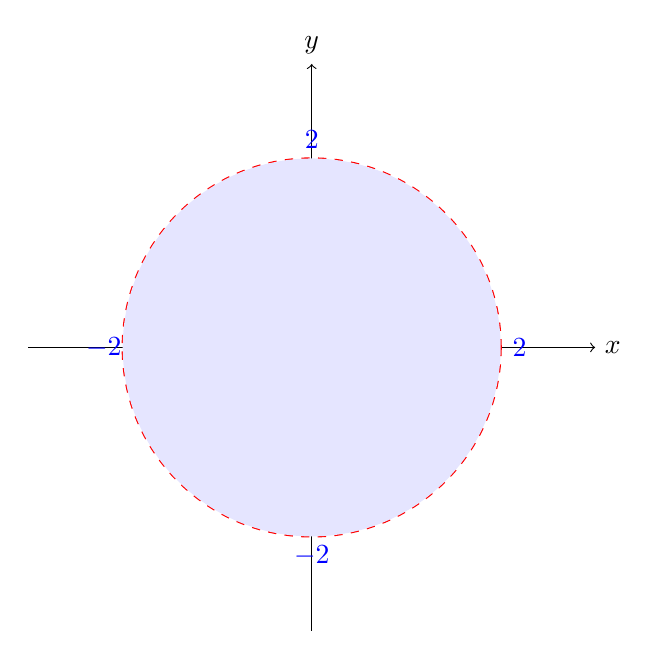
\begin{tikzpicture}[scale=1.2]
% Axes
\draw[->] (-3,0) -- (3,0) node[right] {$x$};
\draw[->] (0,-3) -- (0,3) node[above] {$y$};

% Circle x^2 + y^2 < 4 (dashed)
\draw[thick, red, dashed] (0,0) circle (2);
\fill[blue!10] (0,0) circle (2);

% Labels
\node[blue] at (2.2,0) {$2$};
\node[blue] at (0,2.2) {$2$};
\node[blue] at (-2.2,0) {$-2$};
\node[blue] at (0,-2.2) {$-2$};
\end{tikzpicture}

\vspace{2cm}


\begin{tikzpicture}[scale=1.2, circ/.style={shape=circle, red, inner sep=2pt, draw, node contents=}]
% Axes
\draw[->] (-3,0) -- (3,0) node[right] {$x$};
\draw[->] (0,-3) -- (0,3) node[above] {$y$};

% Parameters
\pgfmathsetmacro{\r}{2}
\pgfmathsetmacro{\xcut}{1.5} % = 3/2
\pgfmathsetmacro{\ycut}{sqrt(\r*\r-\xcut*\xcut)} % = sqrt(7)/2

% Shade and draw the part of the disk that lies in the vertical strip |x|<=3/2

% CLIPPED CIRCLE: Only shows between x = -1.5 and x = 1.5
\begin{scope}
      \clip (-\xcut,-\r) rectangle (\xcut,\r);
  \fill[blue!10] (0,0) circle (\r);
  \draw[thick, red, dashed] (0,0) circle (\r);
\end{scope}

% Draw ONLY the boundary segments x=±3/2 that lie inside the disk
\draw[thick, red] (-\xcut,-\ycut) -- (-\xcut,\ycut);
\draw[thick, red] ( \xcut,-\ycut) -- ( \xcut,\ycut);

\node at (\xcut,\ycut)[circ,label={}];
\node at (-\xcut,\ycut)[circ,label={}];
\node at (\xcut,-\ycut)[circ,label={}];
\node at (-\xcut,-\ycut)[circ,label={}];


% Labels
\node[blue, below] at (\xcut,0) {$\tfrac32$};
\node[blue, below] at (-\xcut,0) {$-\tfrac32$};
\node[blue, right] at (\r,0) {$2$};
\node[blue, above] at (0,\r) {$2$};
\node[blue, left] at (-\r,0) {$-2$};
\node[blue, below] at (0,-\r) {$-2$};
\end{tikzpicture}


\qpart

\qsubpart

By \textup{Definition 3.6 HB Chapter 16 p84 },

let \( x = \frac{3}{2} \) and solve for \( y \) in set B's inequality:
\[ x^{2} + y^{2} < 4 \];

then \( y = \sqrt{2^{2} - (\frac{3}{2})^{2}} = \sqrt{\frac{7}{4}} = \frac{\sqrt{7}}{2} \).
Thus, one closure point is \( (\frac{3}{2}, \frac{\sqrt{7}}{2}) \).

\qsubpart

Closure of set C is:
\[ C1 = \{ (x,y) \in \R^{2} : 2|x| \leq 3 \text{ and } x^{2} + y^{2} \leq 4 \} \]

\bigskip

Interior of set C is:
\[ Int = \{ (x,y) \in \R^{2} : 2|x| < 3 \text{ and } x^{2} + y^{2} < 4 \} \]

\bigskip

Boundary of set C is:
\[ Bd = \{ (x,y) \in \R^{2} : (2|x| = 3 \text{ and } x^{2} + y^{2} \leq 4) \text{ or } (2|x| \leq 3 \text{ and } x^{2} + y^{2} = 4) \} \]

\vspace{2cm}

\qpart

Given the 'mixed' metric \( d \);

\[ d((x_{1},y_{1}),(x_{2},y_{2})) = |x_{1} - x_{2}| + d_{0}(y_{1},y_{2}) \]

With \( d_{0} \) the discrete metric on \( \R \).

By \textup{Definition 2.3 HB Chapter 14 p72}

\[ d_{0}(y_{1},y_{2}) = \begin{cases}
0, \text{ if } y_{1} = y_{2},\\
1, \text{ if } y_{1} \neq y_{2}.
\end{cases} \]

Consider
\[ C = \{ (x,y) \in \R^{2} : 2 \mid x \mid \leq 3 \text{ and } x^{2} + y^{2} < 4 \} \]

Take \( (x_{0},y_{0}) \) to satisfy
\[ 2|x_{0}| \leq 3 \text{ and } x_{0}^{2} + y_{0}^{2} \leq 4 \]

Then if \( x_{0}^{2} + y_{0}^{2} < 4 \) then \( x_{0}^{2} + y_{0}^{2} \in C \) and therefore a closure point.

And if \( x_{0}^{2} + y_{0}^{2} = 4 \) and \( 2|x_{0}| \leq 3 \) then it is possible to choose a sequence
\( (x_{n},y_0) \) with \( x_{n}^{2} + y_{0}^{2} < 4 \) and \( x_{n} \to x_{0} \). As \( y \) stays constant,

\[ d((x_{n},y_{0}),(x_{0},y_{0})) = |x_{n} - x_{0}| \to 0 \]

Hence boundry points are also closure points and the closure of C is:
\[ C1 = \{ (x,y) \in \R^{2} : 2|x| \leq 3 \text{ and } x^{2} + y^{2} \leq 4 \} \]

\end{question}

%Question 6
\begin{question}

    \[ D = \left\{ x\in \R : x = \frac{m}{p} \text{ for some } m \in \N \text{ and } p \text{ prime } \right\} \]

\qpart

\( m \in \N \) is countable, \textup{Definition 6.4 HB Chapter 16 p87}, and 
\( p \in \N \) is countable. Hence \( D \in \Q \), is countable, \textup{Theorem 6.6 HB Chapter 16 p87}.

\bigskip

\qpart

\qsubpart

\begin{proof}
$$\newline

For
\[ y \geq 0 \]
and
\[ r > 0 \]
Hence
\[ y+r > 0 \]

\begin{align*}
\stext{Let \( p \) be a prime number, in the interval}
(yp, p(y + r))\\[8pt]
\stext{The lenght of this interval is}
p(y + r) - yp = pr\\[8pt]
\stext{As \( r > 0 \), and primes are unbounded, there exists a prime \( p \) such that}
pr > 1\\[8pt]
\stext{Hence}
p(y + r) - yp = pr > 1\\[8pt]
\stext{Therefore contains at least one integer \( m \in \N \) }
\stext{Thus}
yp < m < p(y + r)\\[8pt]
\stext{Dividing by \( p \) gives}
y < \frac{m}{p} < y + r\\[8pt]
\stxt{With \( \frac{m}{p} \in D \)}
\end{align*}

Therefore, there exists \[ x = \frac{m}{p} \in D \] such that
\[ y < x < y + r \]

\end{proof}

\vspace{2cm}

\qsubpart

\begin{proof}
$$\newline

To show the \( D \) is dense in \( [0,\infty) \), we need to show that for any
\[ a, b \in [0, \infty) \]
such that
\[ a < b \]
there exists
\[ x \in D \]
such that
\[ a < x < b \]

Let
\[ r = b - a > 0 \]
From part (i), we know that there exists
\[ x \in D \] such that
\[ a < x < a + r \]
But
\[ a + r = a + (b - a) = b \]
Thus
\[ a < x < b \]
and so \( D \) is dense in \( [0, \infty) \).

\end{proof}

\end{question}

%Question 7
\begin{question}

I have watched the tutorial but forgot the date. I have emailed my tutor and was advised to write 
this as a proof of enagement. 

\end{question}

\section{Part B}

%Question 8
\begin{question}

    Question 8 from section B

Let \( R \) be the ring \( \Z[\sqrt{-13}] \)

\qpart

\[ A = \{ s + t\sqrt{-13} : s,t \in \Z, s - t \equiv 0\pmod{7} \} \]

As \( s = t\pmod{7} \) there eisits an integer \( k \) such that,
\[ s = t + 7k \]
Hence,
\begin{align*}
s + t\sqrt{-13} &= (t + 7k) + t\sqrt{-13} \\[8pt]
&= t(1 + \sqrt{-13}) + 7k\\[8pt]
\stext{So}
A \langle 7, 1 + \sqrt{-13} \rangle
\end{align*} 

By \textup{Definition 2.1 HB Chapter 17 p94},

To Show \( A \) is ideal, it must be closed under multiplication by any \( r \in R \).
So we need the product of the generator and \( \sqrt{-13} \) to stay in \( A \).

\begin{align*}
\sqrt{-13}(1 + \sqrt{-13}) &= \sqrt{-13} -13\\[8pt]
\stext{since} -13 &\equiv 1\pmod{7} \\[8pt]
-13 &= 1 -14\\[8pt]
\sqrt{-13} -13 &= (\sqrt{-13} + 1) - 14\\[8pt]
&= (\sqrt{-13} + 1) + 7(-2)
\end{align*}

Since \( (\sqrt{-13} + 1) \in A \) and \( 14 = 2(7) \in A \) it follows that \( A \) 
is closed under multiplication by any element of \( R \) and hence is an ideal.

\vspace{3cm}

\qpart

\[ B = \{ u + v\sqrt{-13} : u,v \in \Z, u + v \equiv 0\pmod{7} \} \]

As \( u = -v\pmod{7} \) there eisits an integer \( k \) such that, 
\[ u = -v + 7k \] 

Hence, 
\begin{align*} 
    u + v\sqrt{-13} &= (-v + 7k) + v\sqrt{-13} \\[8pt] 
    &= v(-1 + \sqrt{-13}) + 7k\\[8pt] 
    \stext{So} 
    B \langle 7, -1 + \sqrt{-13} \rangle
\stext{because \( -1 \) is a unit in \( \Z[\sqrt{-13}] \), therefore we can multiply the second generator by \( -1 \) and it will still generate the same ideal.}
    B \langle 7, 1 - \sqrt{-13} \rangle
\end{align*}

Hence,

\begin{align*}
A & \langle 7, 1 + \sqrt{-13} \rangle \\[8pt]
\stext{and}
B & \langle 7, 1 - \sqrt{-13} \rangle\\[8pt]
\stext{By \textup{Lemma 3.9 HB Chapter 17 p97}, the product of two ideals \(A\) and \( B \)}
AB & \langle 7\cdot 7, 7(1 - \sqrt{-13}), 7(1 + \sqrt{-13}), (1 + \sqrt{-13})(1 - \sqrt{-13}) \rangle \\[8pt] 
& \langle 49, 7(1 - \sqrt{-13}), 7(1 + \sqrt{-13}), 14 \rangle\\[8pt]
\stext{Since the \( \hcf(14, 49) = 7 \) and \( 7(1 - \sqrt{-13}) \) and \( 7(1 + \sqrt{-13}) \) are multiples of \( 7 \) and,}
 7 &= 49 -3(14) \in AB\\[8pt]
\langle 7 \rangle &\subseteq AB\\[8pt]
\stext{hence}
AB & \langle 7 \rangle
\end{align*}



\end{question}


\end{question}

%Question 9
Question 9 from section B
\begin{question}

\[ B_{d}((0,0),1), B_{d}[(0,0),1], \text{ and } S_{s}((0,0),1)   \]

By \textup{Defintion 2.6 HB Chapter 14 p 72}

\qpart

The open ball on metric 
\[ d((a_{1},a_{2}),(b_{1},b_{2})) = 6|b_{1} - a_{1}| + |b_{2} - a_{2}| \]

is given by
\begin{align*}
B_{d}((0,0),1) &= \{ (x,y) \in \R^{2} : d((x,y),(0,0)) < 1 \} \\[8pt]
&= \{ (x,y) \in \R^{2} : 6|x - 0| + |y - 0| < 1 \} \\[8pt]
&= \{ (x,y) \in \R^{2} : 6|x| + |y| < 1 \}      
\end{align*}

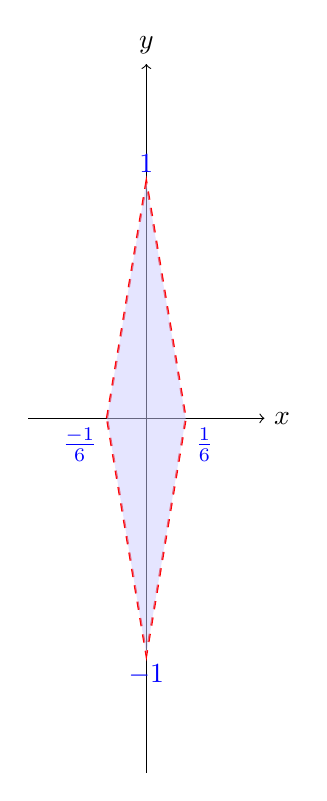
\begin{tikzpicture}[scale=3]
    %axis
    \draw[->] (-0.5,0) -- (0.5,0) node[right] {$x$};
    \draw[->] (0,-1.5) -- (0,1.5) node[above] {$y$};

    %boundry (dashes)
    \draw[thick, dashed, red] (-1/6,0) -- (0,1) -- (1/6,0) -- (0,-1) -- cycle;
    \fill[blue!20,opacity=0.5] (-1/6,0) -- (0,1) -- (1/6,0) -- (0,-1) -- cycle;

    %labels
    \node[blue, below left] at (-1/6,0) {$\frac{-1}{6}$};
    \node[blue, below right] at (1/6,0) {$\frac{1}{6}$};
    \node[blue, above] at (0,1) {$1$};
    \node[blue, below] at (0,-1) {$-1$};
\end{tikzpicture}

The closed ball on metric
\[ d((a_{1},a_{2}),(b_{1},b_{2})) = 6|b_{1} - a_{1}| + |b_{2} - a_{2}| \]

is given by
\begin{align*}
B_{d}[(0,0),1] &= \{ (x,y) \in \R^{2} : d((x,y),(0,0)) \leq 1 \} \\[8pt]
&= \{ (x,y) \in \R^{2} : 6|x - 0| + |y - 0| \leq 1 \} \\[8pt]
&= \{ (x,y) \in \R^{2} : 6|x| + |y| \leq 1 \}      
\end{align*}

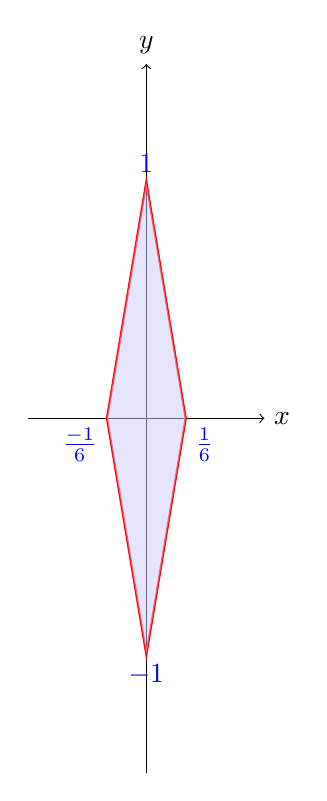
\begin{tikzpicture}[scale=3]
    %axis
    \draw[->] (-0.5,0) -- (0.5,0) node[right] {$x$};
    \draw[->] (0,-1.5) -- (0,1.5) node[above] {$y$};

    %boundry (solid)
    \draw[thick, red] (-1/6,0) -- (0,1) -- (1/6,0) -- (0,-1) -- cycle;
    \fill[blue!20,opacity=0.5] (-1/6,0) -- (0,1) -- (1/6,0) -- (0,-1) -- cycle;

    %labels
    \node[blue, below left] at (-1/6,0) {$\frac{-1}{6}$};
    \node[blue, below right] at (1/6,0) {$\frac{1}{6}$};
    \node[blue, above] at (0,1) {$1$};
    \node[blue, below] at (0,-1) {$-1$};
\end{tikzpicture}

Thh sphere on metric
\[ d((a_{1},a_{2}),(b_{1},b_{2})) = 6|b_{1} - a_{1}| + |b_{2} - a_{2}| \] is given by
\begin{align*}
S_{s}((0,0),1) &= \{ (x,y) \in \R^{2} : d((x,y),(0,0)) = 1 \} \\[8pt]
&= \{ (x,y) \in \R^{2} : 6|x - 0| + |y - 0| = 1 \} \\[8pt]
&= \{ (x,y) \in \R^{2} : 6|x| + |y| = 1 \}      
\end{align*}

\begin{tikzpicture}[scale=3]
    %axis
    \draw[->] (-0.5,0) -- (0.5,0) node[right] {$x$};
    \draw[->] (0,-1.5) -- (0,1.5) node[above] {$y$};

    %boundry (solid)
    \draw[thick, red] (-1/6,0) -- (0,1) -- (1/6,0) -- (0,-1) -- cycle;

    %labels
    \node[blue, below left] at (-1/6,0) {$\frac{-1}{6}$};
    \node[blue, below right] at (1/6,0) {$\frac{1}{6}$};
    \node[blue, above] at (0,1) {$1$};
    \node[blue, below] at (0,-1) {$-1$};
\end{tikzpicture}

\qpart

The open ball on metric
\[ d((a_{1},a_{2}),(b_{1},b_{2})) = (|b_{1} - a_{1}|^{4}  + |b_{2} - a_{2}|^4)^{\frac{1}{4}} \]

is given by
\begin{align*}
B_{d}((0,0),1) &= \{ (x,y) \in \R^{2} : d((x,y),(0,0)) < 1 \} \\[8pt]
&= \{ (x,y) \in \R^{2} : (|x - 0|^{4} + |y - 0|^{4})^{\frac{1}{4}} < 1 \} \\[8pt]
&= \{ (x,y) \in \R^{2} : (|x|^{4} + |y|^{4})^{\frac{1}{4}} < 1 \}      
\end{align*}

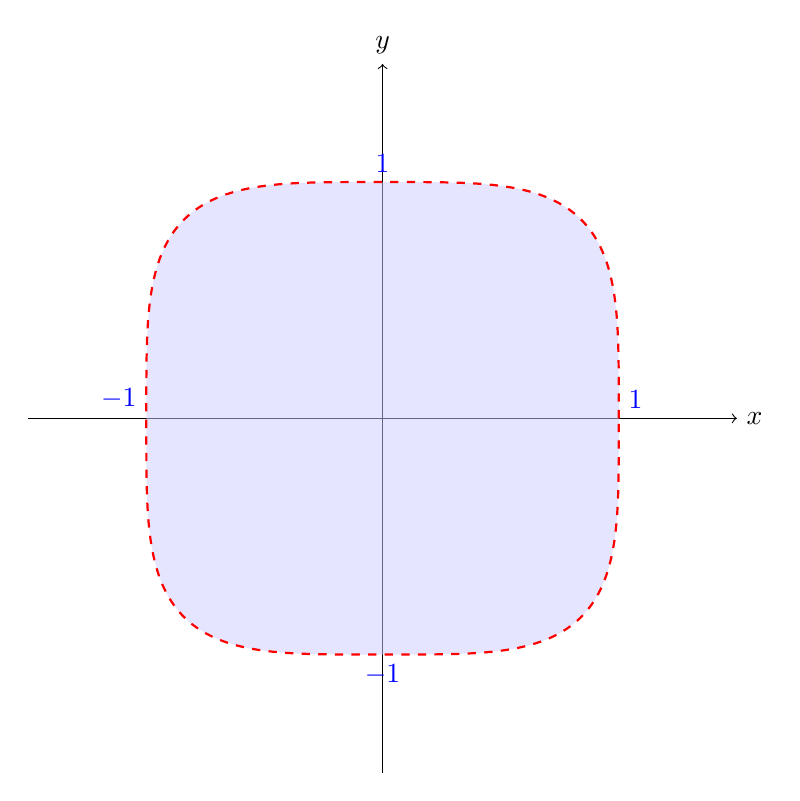
\begin{tikzpicture}[scale=3]
    % axes
    \draw[->] (-1.5,0) -- (1.5,0) node[right] {$x$};
    \draw[->] (0,-1.5) -- (0,1.5) node[above] {$y$};

    % L^4 unit ball boundary: |x|^4 + |y|^4 = 1 (parametric, robust)
    % r(t) = (|cos t|^4 + |sin t|^4)^(-1/4)
    \fill[blue!20,opacity=0.5]
      plot[domain=0:360,samples=240,smooth]
      ({cos(\x)*(abs(cos(\x))^4 + abs(sin(\x))^4)^(-1/4)},
       {sin(\x)*(abs(cos(\x))^4 + abs(sin(\x))^4)^(-1/4)}) -- cycle;

    \draw[thick, dashed, red]
      plot[domain=0:360,samples=240,smooth]
      ({cos(\x)*(abs(cos(\x))^4 + abs(sin(\x))^4)^(-1/4)},
       {sin(\x)*(abs(cos(\x))^4 + abs(sin(\x))^4)^(-1/4)});

    % labels
    \node[blue, above right] at (1,0) {$1$};
    \node[blue, above left] at (-1,0) {$-1$};
    \node[blue, above] at (0,1) {$1$};
    \node[blue, below] at (0,-1) {$-1$};
\end{tikzpicture}

The closed ball on metric
\[ d((a_{1},a_{2}),(b_{1},b_{2})) = (|b_{1} - a_{1}|^{4}  + |b_{2} - a_{2}|^4)^{\frac{1}{4}} \] is given by
\begin{align*}
B_{d}[(0,0),1] &= \{ (x,y) \in \R^{2} : d((x,y),(0,0)) \leq 1 \} \\[8pt]
&= \{ (x,y) \in \R^{2} : (|x - 0|^{4} + |y - 0|^{4})^{\frac{1}{4}} \leq 1 \} \\[8pt]
&= \{ (x,y) \in \R^{2} : (|x|^{4} + |y|^{4})^{\frac{1}{4}} \leq 1 \}      
\end{align*}    

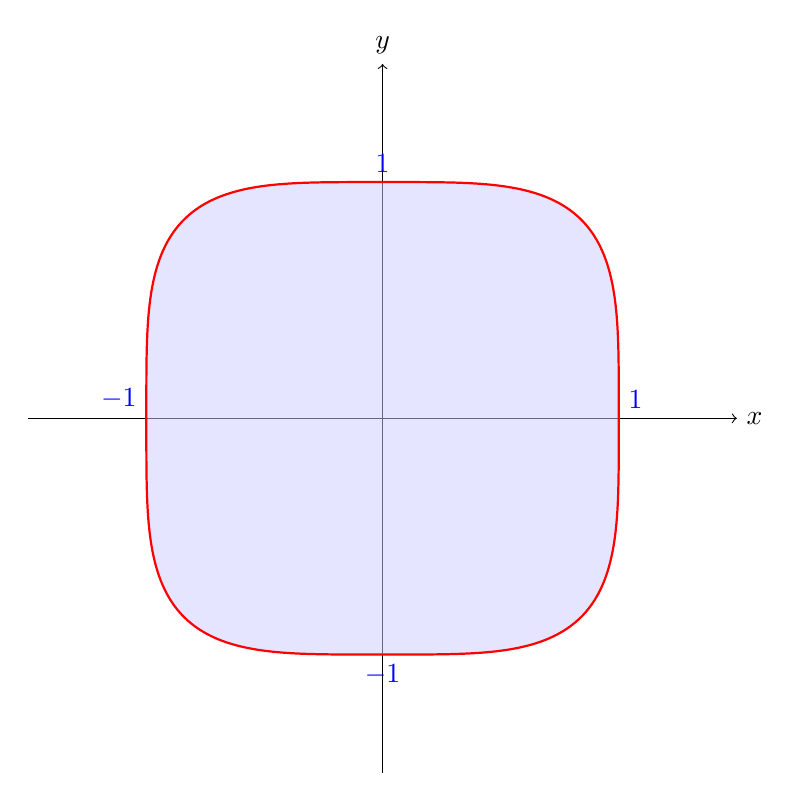
\begin{tikzpicture}[scale=3]
    % axes
    \draw[->] (-1.5,0) -- (1.5,0) node[right] {$x$};
    \draw[->] (0,-1.5) -- (0,1.5) node[above] {$y$};

    % fill the closed ball
    \fill[blue!20,opacity=0.5]
      plot[domain=0:360,samples=240,smooth]
      ({cos(\x)*(abs(cos(\x))^4 + abs(sin(\x))^4)^(-1/4)},
       {sin(\x)*(abs(cos(\x))^4 + abs(sin(\x))^4)^(-1/4)}) -- cycle;

    % boundary (solid)
    \draw[thick, red]
      plot[domain=0:360,samples=240,smooth]
      ({cos(\x)*(abs(cos(\x))^4 + abs(sin(\x))^4)^(-1/4)},
       {sin(\x)*(abs(cos(\x))^4 + abs(sin(\x))^4)^(-1/4)});

    % labels
    \node[blue, above right] at (1,0) {$1$};
    \node[blue, above left] at (-1,0) {$-1$};
    \node[blue, above] at (0,1) {$1$};
    \node[blue, below] at (0,-1) {$-1$};
\end{tikzpicture}

The sphere on metric
\[ d((a_{1},a_{2}),(b_{1},b_{2})) = (|b_{1} - a_{1}|^{4}  + |b_{2} - a_{2}|^4)^{\frac{1}{4}} \] is given by
\begin{align*}
S_{s}((0,0),1) &= \{ (x,y) \in \R^{2} : d((x,y),(0,0)) = 1 \} \\[8pt]
&= \{ (x,y) \in \R^{2} : (|x - 0|^{4} + |y - 0|^{4})^{\frac{1}{4}} = 1 \} \\[8pt]       
&= \{ (x,y) \in \R^{2} : (|x|^{4} + |y|^{4})^{\frac{1}{4}} = 1 \}
\end{align*}        

\begin{tikzpicture}[scale=3]
    % axes
    \draw[->] (-1.5,0) -- (1.5,0) node[right] {$x$};
    \draw[->] (0,-1.5) -- (0,1.5) node[above] {$y$};

    % boundary only (sphere)
    \draw[thick, red]
      plot[domain=0:360,samples=240,smooth]
      ({cos(\x)*(abs(cos(\x))^4 + abs(sin(\x))^4)^(-1/4)},
       {sin(\x)*(abs(cos(\x))^4 + abs(sin(\x))^4)^(-1/4)});

    % labels
    \node[blue, above right] at (1,0) {$1$};
    \node[blue, above left] at (-1,0) {$-1$};
    \node[blue, above] at (0,1) {$1$};
    \node[blue, below] at (0,-1) {$-1$};
\end{tikzpicture}

\qpart

The open ball on metric
\[ d((a_{1},a_{2}),(b_{1},b_{2})) = d_{0}(a_{1},b_{1}) + 6|b_{2} - a_{2}| \]

is given by
\begin{align*}
S_{s}((0,0),1) &= \{ (x,y) \in \R^{2} : d((x,y),(0,0)) < 1 \} \\[8pt]
&= \{ (x,y) \in \R^{2} : d_{0}(x,0) + 6|y - 0| < 1 \} \\[8pt]
&= \{ (x,y) \in \R^{2} : d_{0}(x,0) + 6|y| < 1 \}   
\end{align*}

\begin{tikzpicture}[scale=3]
    %axis
    \draw[->] (-0.5,0) -- (0.5,0) node[right] {$x$};
    \draw[->] (0,-1) -- (0,1) node[above] {$y$};

    %boundry (solid)
    \draw[dashed, thick, red] (0,-1/6) -- (0,1/6);
    
    %labels
    \node[blue, right] at (0,1/6) {$\frac{1}{6}$};
    \node[blue, right] at (0,-1/6) {$\frac{-1}{6}$};
  
\end{tikzpicture}

The closed ball on metric
\[ d((a_{1},a_{2}),(b_{1},b_{2})) = d_{0}(a_{1},b_{1}) + 6|b_{2} - a_{2}| \] is given by
\begin{align*}
B_{d}[(0,0),1] &= \{ (x,y) \in \R^{2} : d((x,y),(0,0)) \leq 1 \} \\[8pt]
&= \{ (x,y) \in \R^{2} : d_{0}(x,0) + 6|y - 0| \leq 1 \} \\[8pt]
&= \{ (x,y) \in \R^{2} : d_{0}(x,0) + 6|y| \leq 1 \}   
\end{align*}    

\begin{tikzpicture}[scale=3]
    %axis
    \draw[->] (-0.5,0) -- (0.5,0) node[right] {$x$};
    \draw[->] (0,-1) -- (0,1) node[above] {$y$};

    %boundry (solid)
    \draw[thick, red] (0,-1/6) -- (0,1/6);
    \fill[blue!20,opacity=0.5] (0,-1/6) -- (0,1/6) -- cycle;
    
    %labels
    \node[blue, right] at (0,1/6) {$\frac{1}{6}$};
    \node[blue, right] at (0,-1/6) {$\frac{-1}{6}$};

\end{tikzpicture}

The sphere on metric
\[ d((a_{1},a_{2}),(b_{1},b_{2})) = d_{0}(a_{1},b_{1}) + 6|b_{2} - a_{2}| \] is given by
\begin{align*}
S_{s}((0,0),1) &= \{ (x,y) \in \R^{2} : d((x,y),(0,0)) = 1 \} \\[8pt]
&= \{ (x,y) \in \R^{2} : d_{0}(x,0) + 6|y - 0| = 1 \} \\[8pt]
&= \{ (x,y) \in \R^{2} : d_{0}(x,0) + 6|y| = 1 \}   
\end{align*}

\begin{tikzpicture}[scale=3]
    %axis
    \draw[->] (-0.5,0) -- (0.5,0) node[right] {$x$};
    \draw[->] (0,-1) -- (0,1) node[above] {$y$};

    %boundry (solid)
    \draw[thick, red] (0,-1/6) -- (0,1/6);
    
    %labels
    \node[blue, right] at (0,1/6) {$\frac{1}{6}$};
    \node[blue, right] at (0,-1/6) {$\frac{-1}{6}$};
\end{tikzpicture}



\end{question}


\end{document}